\chapter{Introduction}

\ignore{\hl{General: - Coherencia tiempos verbales - Coherencia protein-ligand - Asegurarse que siempre es
PELE++ (post rewrite) }}

Human biology seats in a weak equilibrium. The breakdown of this homeostasis, whether it is because of external agents or deficiencies in the internal regulations, produces illness and death. Therefore, it is not surprising that, throughout its history, humankind has always been looking for treatments and medicines to fight disease. 
Today, more than ever before, we need to keep perfecting health methods. Industrial excesses and lax laws are creating a hostile environment that affects us directly or through the food chain in unexpected ways. Also, the same advances that have allowed the rise of the world's population life expectancy \cite{who_world_????} are being put to the test to cure the increasing number of aging-related illnesses that reduce our quality of life.

\section{The innovation crisis in pharmaceutical industry}

Nowadays, the role of discovering and manufacturing new and better drugs is being played mainly by the pharmaceutical industry. With a 3.9\% of the gross value added in manufacturing worldwide in 2011 \ignore{\hl{an updated document (2015) exists, but it only contains info up to 2012 (good maps for defense); Gross Value Added es equivalente al PIB}} \cite{ostwald_measuring_2013}, more than 690,000 direct employees in Europe (2013) \cite{efpia_pharmaceutical_2014} and more than 810,000 in the United States of America (USA) (2013) \cite{phrma_2015_2015}, its economical importance is out of doubt. Most big pharmaceutical companies have good financial results and are able to attract investors. However,these good results are mainly because of their incremental innovation model, that is, their ability to improve old products \cite{kristopher_hult_should_????}. This is an efficient strategy, since it can help milden the profit loss coming from expiring patents at a time when consumers tend to buy generics over brand name drugs\footnote{The balance increased from 49\% in 2000  to 88\% in 2013 \cite{phrma_2015_2015}.}. 

However, if we focus on an innovation indicator like the number of NMEs (New Molecular Entities) approved every year by the USA's Food and Drug Administration\footnote{ All data refers to USA agencies unless otherwise stated.}, the pharmaceutical industry does not look so  prosperous. The number of approved NMEs has been very low during the last decade (with an average of 24 per year \cite{cder_2013_2014}).This is a matter of concern, since , the cost of marketing one of these drugs has increased three times in the same amount of time. Also, the drug development time span has not shortened and it usually lasts 15 years \cite{dimasi_price_2003}, but can exceed 30 years \cite{goozner_800_2004}. The discovery of a single NME is becoming more difficult and costly, and the revenues returned from them rarely exceed Research and Development (R\&D) investments. That is why, currently, the pharmaceutical industry is considered to be faced with a deep innovation crisis.

\subsection{Possible causes of the crisis}

	Numerous efforts have been made to understand the causes of this crisis in order to improve R\&D efficiency and effectiveness. From what is known, the main problem is not the lack of investments, since the annual spending in R\&D has been around \$40-\$50 billion \cite{phrma_2015_2015, paul_how_2010} during the last ten years. Indeed pharmaceutical companies reinvest a 12.4 per cent of gross domestic sales on R\&D, of which 9.3 to 12.4\% (1.2 / 2.4\% of total) go to fundamental research \cite{light_demythologizing_2011}.

\begin{figure}
\fittopageimage{NMECost}
\caption{Cost and time needed to develop and market one NME (including failures). Cost data were obtained from (in plot order) \cite{mestre-ferrandiz_rd_2012} \cite{phrma_2015_2015} \cite{dimasi_price_2003} \cite{tibco_transforming_????} \cite{peter_gwynne_pharmaceutical_????} \cite{tibco_transforming_????}  \cite{paul_how_2010} \cite{phrma_2011_2011} \cite{oconnor_football_????} \cite{dimasi_cost_2015} \cite{mullin_cost_????}. Time data were obtained from \cite{dreyfus_keeping_????} \cite{dreyfus_keeping_????} \cite{peter_gwynne_pharmaceutical_????} \cite{paul_how_2010}.}
\label{fig:drug_cost}
\end{figure}

Possible causes of the innovation problem include \cite{hughes_innovation_2007}:

\begin{itemize}

\item The increasingly difficult requirements from regulatory agencies to accept new drugs. New standards of safety make clinical trials longer and more costly.

\item The ``saturation of low hanging fruits'' theory, which says that pharmaceutical industry has already discovered all that is possible with our current knowledge.

\item R\&D teams give a sharp focus to revolutionary instead of evolutionary technologies. For instance, the use of genomics-based candidates was so promising that was prioritized over clinically validated drug targets. Still, the repercussions of including revolutionary technologies in pharmaceutical pipelines are not always negative. For example PCR\footnote{Polymerase Chain Reaction} (1983) for DNA\footnote{Deoxyribonucleic acid} replication or gene chips for RNA\footnote{Ribonucleic acid } in the early 1990s allowed researchers to perform more and faster experiments.  

\item Pharmaceutical companies are extremely big, and they spend great amounts of resources on non-productive work.
\end{itemize}

\subsection{Solutions from the pharmaceutical industry }

Pharmaceutical companies have reacted to this situation immediately in order to improve the outcome of their R\&D investments. One of the consequences has been the forge of strategic alliances (especially with biotechnology firms) or even company mergers\footnote{ For instance, the two giants Pfizer and Allergan, have entered into a merger agreement (announced on the 23th of November of 2015), after several hostile takeover bids to AstraZeneca in 2014.}. The industry has also changed its marketing strategies in an attempt to overcome this delicate situation. For instance focusing on rare diseases, or opting for chronic diseases instead of acute diseases make clinical trials more challenging but give good economic results in the long term. 
Finally, drug repurposing seems a good solution as it can reduce the costs of bringing a drug to the market by almost 40\% \cite{chong_new_2007}.

Special attention has been paid to boosting the efficiency of the drug discovery pipeline steps, as this has direct repercussion on the final cost and on the time invested on the drug . For instance, an outsourcing of early steps such as screening, lead identification or lead optimization has shown to decrease the total costs noticeably. Interestingly, if several companies share the same service providers, they will act as  knowledge and expertise exchange nodes, which seems to be a very beneficial side effect in such a hermetic environment . 

\section{The drug discovery pipeline }

The drug discovery pipeline can be divided into two consecutive main phases. In the first one, the aim of researchers is to understand the illness and find a molecule that can cure it (or, at least, improve its symptoms). During the second main phase, which starts right after regulatory agency clearance, the drug is tested in human patients. 

Nowadays Bioinformatics and Computational Biology software play an important role in the discovery process\footnote{The success of Shr\"{o}dinger is a good example of the increasing importance of computational methods in drug discovery. In 2015 they signed a \$120M deal with Sanofi (with tasks including target analysis, validation, lead identification and lead optimization). More recently (2016) they have entered a research collaboration agreement with Pfizer.}. It is hard to quantify the  impact of software on efficiency because, unfortunately, there are few studies on this topic. However, it is quite obvious that the improvements made on this software would also lead to improvements in the overall effectiveness of the pipeline. 

The phases of the pipeline are:
\begin {enumerate}
\item Discovery process
\begin {description}
\item [Pre-discovery] The goal of this phase is to study a disease in order to understand its causes. This phase is usually neglected in pharmaceutical industry reports because of two main factors. First, the time and budget needed are often very variable and this phase generally contributes to drug discovery in the long term. Second, this kind of research is usually performed at non-corporate tax-funded institutions, such as universities or government research centers, and do not have a direct impact on companies budgets. Fostering basic research and the technology transfer between these institutions and the industry is of utmost importance in order to shorten the time of this phase.
\item [Target identification] During this phase, a druggable molecule involved in the disease, usually a protein, is searched . Improvements in this stage come from the use of gene chips and bioinformatics techniques, as well as proteomics \cite{cutler_proteomics_2015}. The sequencing of the human genome also seemed to be an abundant source of drug targets \cite{ grenet_significance_2001, hopkins_druggable_2002}, but, in general, it has not met the initial expectations yet  \cite{garnier_rebuilding_????}. 
\item [Target validation] During this process, the previous target is tested in single cells and animal models. In-vitro validation can be performed by disrupting target expression through the use of  gene knockouts. 
\item [Lead identification] At this point, researchers look for the chemical leads (small drug-like molecules capable of altering the function of the target proteins) and early pharmacokinetics tests (ADME/Tox\footnote{Absorption, Distribution, Metabolism, Excretion and Toxicological}) are performed. This includes the target-to-hit phase, a preliminary screening to filter non-active compounds, and the hit-to-lead phase, a secondary screening where the compounds with the higher potential to become a drug are chosen. High-throughput screening (HTS) and virtual high throughput screening (VHTS) supported by chemoinformatics seem to help speed up this phase. 
\item [Lead optimization] Leads are further optimized to act as a non-toxic therapeutic drug. Rational drug design and combinatorial chemistry work can be used to improve the  properties of the drug candidate.
\item [Preclinical testing] Drug toxicity is determined using in-vitro and in in-vivo (animal models) experiments.
\end {description}

\item Development process
\begin{description}
\item [Phase 1 clinical trial] Initial tests in healthy volunteers (20-100).
\item [Phase 2 clinical trial] Test in a small group of patients (100-500).
\item [Phase 3 clinical trial] Safety and efficacy tests in a large group of patients (1000-5000).
\item [Phase 4 monitoring] After this steps the drug is commercialized, but it is still monitored in search of possible undocumented side effects.
\end{description}
\end {enumerate}

Several new technologies have been used to lower the cost and time required for clinical trials. Genomics, for instance, would allow subdividing patients according to their drug response, and pharmacogenetics and expression pharmacogenomics can enhance the predictions of patient's drug response by analyzing their DNA variability or determining the levels of gene expression.
The use of collaborative management software in clinical trials has shown to have positive effects on the efficiency as it makes researchers less prone to commit errors.

\begin{sidewaysfigure}
    \centering
    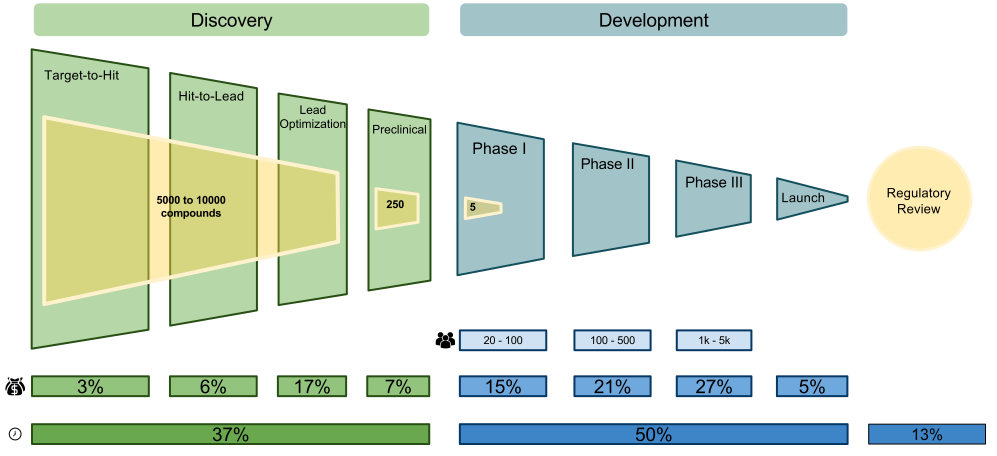
\includegraphics[width=\textwidth,height=\textheight,keepaspectratio]{DrugDevPipeline.pdf}    
    \caption{Drug discovery pipeline phases (pre-discovery and target identification phases have been omitted). The number of compounds used at each step \cite{efpia_pharmaceutical_2014, phrma_2013_2013}, the number of people involved in the clinical trials \cite{phrma_2013_2013}, the percentage of the total development cost per phase \cite{paul_how_2010}, and the percentage of time invested in each phase \cite{dimasi_cost_2015, light_demythologizing_2011, austin_research_2006} are illustrated.}
    \label{fig:drug_dev_pipeline}
\end{sidewaysfigure}

\section{HTS and VHTS}

The early steps of the pipeline are crucial for the success. Target selection, for instance, is one of the most important determinants of R\&D productivity as an error during this phase can potentially compromise the entire process.  

The lead identification step is a very sensitive point too. This step is often performed using HTS. With this technique, lead molecules are identified through automated individual chemical assays using libraries of millions of compounds. Almost a 40-45\% of the drugs currently being tested in human clinical trials come from HTS systems. This is more than four times the percentage found ten years ago \cite{peter_gwynne_pharmaceutical_????}.

Instead of finding hits using experimental assays, screening experiments can also be conducted in-silico through VHTS protocols. These high-speed computer screenings consume only a small percentage of the R\&D costs and time and can potentially save up to one year and 15\% of the total development cost (according to the Boston Consulting Group \cite{tollman_revolution_2001}).

\subsection{How does VHTS work?}

In order to start the VHTS process, researchers first need to obtain libraries of compounds. The following steps will vary depending on the approach adopted. 
The first one is ligand-based virtual screening (LBVS). It rests on the idea that molecules with similar structures have similar properties. It uses the information of  compounds known to bind the protein and does not need the structural data of the target \cite{dror_novel_2009, clark_prospective_2009}. It may use Quantitative Structure-Activity Relationship methods, pharmacophore modeling (``the largest common denominator'') and database mining. 
The second approach, that is structure-based virtual screening (SBVS), needs the tridimensional structure of the target and uses docking algorithms to select the drugs that bind best. 
The choice of one method or the other depends on the availability of data and on the type of problem. LBVS methods are still dominating the VS field because lead information is usually more easily available than structural information \cite{bajorath_integration_2002}. However SBVS is gaining reputation, probably because nowadays there is a huge amount of structural data available for researchers (e.g. the Protein Data Bank (PDB) \cite{berman_protein_2000} stores more than 100k structures, and in-house industry resources also store extensive data), and it looks to be increasing at a good pace thanks to the advances of structure determination techniques. Moreover, SBVS is able to find allosteric binding sites, which is more difficult in LBVS approaches \cite{tanrikulu_pseudoreceptor_2008}. SBVS and LBVS are not mutually exclusive and can improve final results if used together \cite{schaerfe_critical_2011, gil-redondo_vsdmip_2009, prathipati_integration_2015}.

The phases of SBVS usually are:

\begin{description}

\item [Prefiltering] Libraries are prefiltered using their ADME/Tox properties and a physicochemical profile (if a lead profile is available).
Binding site discovery: When crystal structures with bound ligands are not available, cavities can be located computationally using either geometric approaches (e.g. fpocket \cite{le_guilloux_fpocket_2009}), grid-based approaches (e.g. LigSite \cite{huang_ligsitecsc_2006}) or energy-based approaches.

\item [Docking] A high throughput docking over thousand to millions \cite{tuffery_flexibility_2012} of compounds is performed. Each single compound is positioned into the target's previously discovered binding pockets using docking software (e.g. DOCK \cite{kuntz_geometric_1982}, AUTODOCK \cite{morris_distributed_1996, morris_autodock4_2009}, GOLD \cite{jones_molecular_1995}, GLIDE \cite{friesner_glide_2004}, FlexX \cite{rarey_fast_1996}, ARTIST \cite{yun_artist_2006}, ICM \cite{abagyan_icm_1994}, and Surflex-Dock \cite{jain_surflex_2003} among others).

\item[Scoring] Finally the poses are ranked using a scoring function, and the best results are kept. These scoring functions include: force field scoring, empirical scoring, knowledge-based scoring and consensus scoring (which uses more than one scoring function in order to balance their errors). The calculation of binding free energies as a scoring function by using, for example, endpoint (MM/PBSA\footnote{Molecular Mechanics (combined with) Poisson-Boltzmann Surface Area}), pathway (PMF\footnote{Potential of Mean Force}, Metadynamics) or free energy perturbation methods is more rigorous, but also more computationally expensive \cite{mobley_binding_2009, weis_ligand_2006} and barely used. 

\end {description}

VHTS works as a filtering mechanism that benefits the following stages by reducing the number of compounds to be tested experimentally\footnote{This need has been lately acknowledged with the approval of the 4-year project ADDoPT (Advanced Digital Design of Pharmaceutical Therapeutics) in the UK. One of its goals is to improve the productivity of drug discovery processes through the  early detection of non-viable drugs by using mainly computer tools and big data approaches. The academia and the industry (including big pharmaceutical companies such as AstraZeneca, Bristol-Myers Squibb, GlaxoSmithKline and Pfizer) will cooperate in order to bring the process to a successful conclusion.} (e.g. inactive compounds). However, its use can become a burden if too many false positives are generated, thus ``contaminating'' the pipeline; errors will be paid in next steps at a high cost \cite{moustakas_application_2007}.
That is why it is desirable and more productive to ``fail fast'' and unambiguously. The sources of error in SBVS are numerous: incorrect protonation \cite{totrov_flexible_2008}, incorrect assignment of side chain rotamers, low sequence identity in homology modelling (if the structure is not available), absence of water in the binding site \cite{de_beer_role_2010}, incorrect/no handling of flexibility or, simply, inaccuracies of the docking procedure or in the scoring functions. As a consequence, it is still safer to use SBVS as a complement \cite{doman_molecular_2002} to empirical screening rather than as a complete replacement (e.g. to increase hit-rate of HTS). 

\subsection{Fast docking software}

The keystone of the SBVS process is the high throughput docking software. Docking is one of the most significant challenges of computational biology and represents an area of intense academic research \cite{hartshorn_diverse_2007}. Docking algorithms can be classified in several categories, depending on the types of molecules (protein-protein and protein-ligand docking), the treatment of flexibility (flexible ligand, receptor or both), or the algorithmic details (matching or simulation). Given receptor and ligand molecules, the goal of a docking program is to predict if they interact and find their relative positions and conformations in order to generate the resulting complex. 

VHTS-compatible docking software must be fast. The time it works with each compound cannot exceed a few seconds, as libraries may contain thousand to millions of them \cite{schaerfe_critical_2011}. The combinatorial explosion of possible conformations/poses due to the enormous number of internal and external degrees of freedom involved makes it hard to perform a systematic exploration of the solution space. As a consequence, many simplifications must be done in order to attain reasonable execution times. To this end, the docking problem usually becomes an optimization problem over certain fitness function where a rigorous simulation of the biophysical properties of the system, as well as  the handling of ligand and receptor flexibility, is often sacrificed.

\section{Flexibility}

\subsection{Flexibility and binding}

Flexibility is known to play a major role in molecular recognition processes and is a long-studied topic. Nowadays, we know that it contributes to favorable changes in the binding free energy \cite{verkhivker_complexity_2002} by optimizing the noncovalent interactions between the receptor and the ligand, or by increasing the entropy upon binding by releasing interfacial water and increasing flexibility in parts of the protein or ligand \cite{zavodszky_side-chain_2005}. However, the importance of flexibility has not always been present in binding theories. Models like Fisher's ``lock and key'' \cite{fischer_einfluss_????} (1984), described binding as an entirely rigid interaction in which ligands and receptors must be complementary in shape in order to bind. This model prevailed for more than 60 years until Koshland \cite{koshland_application_1958} formulated its induced fit hypothesis in 1959. In this second model, the ligand is able to produce a deformation in the receptor's active site: complete complementarity is not needed for binding to happen. Another hypothesis, the conformational selection model \cite{monod_nature_1965, rubin_nature_1966}, asserts that all possible conformers of the receptor coexist in solution, including the binding one. The interaction with the ligand produces a population shift towards the binding conformation. The consequences of this model can affect drug design strategies as the knowledge of these relative populations could be used to create drugs with different degrees of binding affinities. 

Currently, both the induced fit and conformational selection models are accepted. Both agree on the fact that binding is a dynamic event where ligand and receptor may change their structures dynamically. Although these models may not be complete, as both are defied by intrinsically disordered proteins (IDPs\footnote{A fourth model "coupled folding and binding" \cite{wright_linking_2009}}), experimental evidences support them (e.g. the findings on HIV-1 protease \cite{wlodawer_inhibitors_1998}, DHFR \cite{bystroff_crystal_1991}  or aldose reductase \cite{wilson_refined_1993} ); this may mean that they are not exclusive. 

\subsection{Flexibility models} 

Neglecting the treatment of flexibility reduces the degrees of freedom of the search space dramatically, thus lowering the time needed to find solutions. However it can severely limit the accuracy of results. Some studies, for instance, show that the consequences of incorrectly treating flexibility drive a success rate drop of  \around25\%-55\% in binding simulations  \cite{erickson_lessons_2004} being this drop proportional to the number of rotatable bonds of the ligand and correlated with the degree of the protein movement in the active site. In order to improve the accuracy of docking software, a restricted treatment of flexibility must be applied, trying to reach a good compromise between a robust theoretical treatment and computational performance. 

\subsubsection{Molecular Dynamics and flexibility}

The best-known method to sample the flexibility of ligands and receptors is molecular dynamics (MD). In MD, the positions of the particles of the system are predicted by integrating Newton's equations of movement. This method offers a detailed vision of the dynamics of molecules, allowing to understand how systems evolve at atomic level. 

Despite its renown, MD is not completely flawless. For instance, the force fields it uses (see Fig. \ref{fig:md_force_field}) are known to be biased towards certain types of secondary structures \cite{yildirim_benchmarking_2011, cino_comparison_2012}, and it has been reported that simulations can end trapped into sink free energy states \cite{lange_scrutinizing_2010, raval_refinement_2012}, reducing the sampling quality. Also, the discretization error of integrators advises against running single long simulations in favour of running multiple short ones \cite{lange_scrutinizing_2010, raval_refinement_2012}. Despite this, MD simulations have shown to have a good correlation with experiments (for example in comparisons with Residual Dipolar Coupling data \cite{lin_evaluating_2011}) and has been successfully used on many occasions to unveil molecular mechanisms that could not be studied in other manners. The reviews of Karplus \cite{karplus_molecular_2002}, Dodson \cite{dodson_molecular_2008} and Dror \cite{dror_biomolecular_2012} illustrate many of these success stories. 


\begin{figure}
\fittopageimage{ForceField}
\caption{Example of the interactions described by a force field. From them the potential energy of the system ($U = E_{bond} + E_{angle} + E_{torsion} + E_{nb} $) as well as the forces, accelerations and velocities of each single particle (atom) can be calculated.}
\label{fig:md_force_field}
\end{figure}

The integration step in MD must be small enough to guarantee the algorithm's stability and is frequently set on the femtosecond scale. Given that functional changes, which may be related to binding mechanisms, often occur at the $\mu$s/ms scale, obtaining an informative simulation requires computing a considerable number of steps. Besides, the atomic detail of simulations, which usually includes an explicitly modeled solvent, means that studied systems have a huge amount of particles, making the calculation of each step harder. These are the main reasons why MD is such a computationally demanding method. 

Even with the current algorithmic and hardware progress (that includes the intensive use of accelerators), calculations cannot routinely exceed the $\mu$s total time. The construction of single-purpose dedicated-hardware machines (e.g. FASTRUN \cite{fine_fastrun_1991}, MD Engine \cite{shinjiro_toyoda_development_1999}, MDGRAPE \cite{taiji_protein_2003} and ANTON \cite{shaw_anton_2008}) has allowed researchers to perform longer simulations more easily. An example of this is a recent work by Shan \cite{shan_how_2011},  who has calculated a 20 microsecond simulation showing the free diffusion and binding process of dasatinib and the kinase inhibitor PP1 with Src kinase. Unfortunately, these specialized computers are usually not publicly accessible, and even if they were, the pace at which these machines produce results is still impractical for high throughput methodologies like VS\footnote{With the exception of generating ensembles for "multiple receptor conformations" methods \cite{gorfe_functional_2005, wong_molecular_2005}}. 

Derived methods aiming to speed MD simulations, like replica exchange, are still too slow to be applied in VS protocols. The need to overcome these computational limitations led to the creation of the first rigid ligand / rigid receptor algorithms. However, the need for some forms of computationally lightweight flexibility was acknowledged shortly afterwards, giving place to other well-known techniques such as:

\begin {description}
\item [Incremental construction] A rigid part of the ligand is docked first and then the flexible elements are incrementally added so that the ligand adapts to the binding site. Ex. GROWMOL \cite{bohacek_growmol_1999}.

\item [Multiple conformations] Can be applied to both ligand and receptor. In the case of the ligand, new conformations can be obtained by sampling the angles of rotatable bonds and keeping the lower energy solutions, using them for the docking. The main problem is that the complexed ligand is not always in a low energy state \cite{hurst_flexible_1994, nicklaus_conformational_1995}. In the case of a protein receptor, different conformations can be obtained from Nuclear Magnetic Resonance (NMR) or X-ray structure determination experiments. 
\end {description}

Other types of methods perform a conformational search in order to sample different receptor and ligand structures. Some of these methods are simulated annealing (Yue's algorithm \cite{yue_distance-constrained_1990}), Genetic Algorithms (ex. DARWIN \cite{taylor_darwin_2000}), tabu search (Ex. PRO\_LEADS \cite{baxter_flexible_1998}) and path planning (MIAX \cite{del_carpio-munoz_miax_2002}).

Due to their inherent flexibility, the representation of side chains is a challenge on its own. Several techniques have been proposed. For example, the "soft receptors" method allows the interpenetration between atoms to a certain extent \cite{jiang_soft_1991}. It is more frequently  used in fully rigid docking setups. Another possibility is the use of rotamer libraries. This is a systematic method in which a collection of possible rotamers for side chain torsional angles is randomly or heuristically applied.

\subsubsection{Normal Mode Analysis (NMA) as an alternative}

At this point, it may be clear that a reasonable compromise between the correct modeling of flexibility and its computational requirements must be found: accuracy and detail in the representation of flexibility have an expensive price in CPU\footnote{Central Processing Unit} cycles, but if a less accurate treatment of flexibility is chosen, the simulation can be so inexact to become useless. NMA-based methods might offer a reasonable trade-off, since they add flexibility in the receptor at a low computational cost. 

The basis of NMA \cite{goldstein_classical_1950} is to simplify the potential energy surface by means of a harmonic approximation. To this end, a potential well is built around a stable conformation (here with general coordinates $q$). The molecule is represented by a set of coupled harmonic oscillators and motion is restricted to small fluctuations around that single minimum. The Taylor expansion to the second order of the potential and kinetic energy around the minimum is:

\begin{equation}
V = V_0 + \sum^N_{\alpha=1}\left (  \frac{\partial V}{\partial q_\alpha} \right )_0 q_\alpha + \frac{1}{2} \sum^N_{\alpha=1} \sum^N_{\beta=1} \left ( \frac{\partial^2 V}{ \partial q_\alpha \partial q_\beta} \right )_0 q_\alpha q_\beta + \dotsb
\end{equation}

\begin{equation}
K = K_0 + \sum^N_{\alpha=1}\left (  \frac{\partial K}{\partial \dot{q}_\alpha} \right )_0 \dot{q}_\alpha + \frac{1}{2} \sum^N_{\alpha=1} \sum^N_{\beta=1} \left ( \frac{\partial^2 K}{ \partial \dot{q}_\alpha \partial \dot{q}_\beta} \right )_0 \dot{q}_\alpha \dot{q}_\beta + \dotsb
\end{equation}

Under the assumption of equilibrium, the kinetic and potential energy depend only on the second order terms.

From the resulting Hessian $H$ (where $H_{\alpha\beta} = \frac{\partial^2 V}{ \partial q_\alpha \partial q_\beta }$) and metric tensor $K$ where $K_{\alpha\beta} = \frac{ \partial^2 K}{ \partial \dot{q}_\alpha \partial \dot{q}_\beta } $ the equations of motion can be derived from Lagrange's equation, with the Lagrangian $L = ­K - V$, so that:

\begin{equation}
- \sum_{\beta}^N H_{\alpha \beta} q_\beta = \sum_{\beta}^N K_{\alpha \beta}  \dot{q}_\beta
\end{equation}

The N harmonic solutions to the equations of motion ($q_\alpha = \sum_k^N A_{\alpha k } \alpha_k cos(\omega_k t + \phi_k)$ ) can be calculated by solving the eigenproblem:

\begin{equation}
KA\Lambda = HA
\label{eq:eigenproblem}
\end{equation}

where $A$ and $\Lambda$ are the eigenvector and eigenvalues matrices respectively. The resulting modes are an orthonormal basis of all possible deformations of the molecule around the equilibrium structure. For sufficiently small displacements, the motion of the particles in the system is proportional in amplitude to the magnitude of the eigenvectors and its frequency is proportional to the square root of the eigenvalue. Also, each eigenvalue represents the energetic cost of displacing the system by one length unit along its eigenvector. In general, we are only interested in the subset of modes of lower frequencies i.e. the ones that require less energy, as this slower but wider displacements are usually the ones encoding functional information. 

\subsubsection{ANM}
\label{sec:anm_is_good}

In 1996, Tirion \cite{tirion_large_1996} introduced an NMA model where the molecule is modeled as an EN of Hookean springs of equal strength with potential:

\begin{equation}
V = \sum _{\alpha, \beta} \frac {k}{2} (r_{\alpha\beta}) ^2
\end{equation}

One of the advantages of the simplification of the potential is that, unlike regular NMA,  it does not need to minimize the initial structure to fulfil the assumption of equilibrium: the initial description of the network is already in equilibrium. 

Bahar and coworkers \cite{bahar_direct_1997} extended the model by using only the $C_\alpha$ atoms to represent each residue in an isotropic NMA version. Moreover, the number of atomic interactions was reduced by using a cutoff distance. They showed that, even with these dramatic simplifications, the beta factors derived from the new model were in good agreement with experiments. The model was further improved by Atilgan \textit{et al.} \cite{atilgan_anisotropy_2001}, who used it to extract anisotropic information from the fluctuations. This development, and more generally the NMA models using elastic networks and coarse-grained representations, are also known as Anisotropic Network Models (ANM, see Fig. \ref{fig:anm_4ake_app}).

Most of the efforts to enhance the model have focused on finding a definition of force constants that is able to improve the modeling of the atomic interactions. First attempts come from Hinsen's work \cite{hinsen_analysis_1998}, whose distance-dependent force with exponential decay was fitted using the AMBER force field. More recent studies include the analysis of different formulations for the force constant \cite{sen_optimizing_2005} and MD-based parameterizations \cite{orellana_approaching_2010}. 

The most important computational improvements of ANM come from the use of a cutoff and from the coarse-grained representation. The cutoff reduces the number of iterations needed to calculate the Hessian and the reduction of degrees of freedom from the reduced representation makes it smaller and easier to diagonalize. Since the Hessian calculation represents  the computational bottleneck, finding efficient methods to diagonalize it has been the focus of several research projects. These efforts have resulted in the creation of new algorithms such as the RTB (Rotational-Translational Block) \cite{tama_building-block_2000} or BNM (Block Normal Mode) \cite{li_coarse-grained_2002}, as well as more efficiently parallelizable techniques using the Krylov subspace and Cholesky factorization \cite{lopez-blanco_imod_2011}. Besides, the use of mass-weighted coordinates further simplifies calculations by avoiding the need to calculate the Kinetic tensor (the equation $\hat{H} \hat{A} = \hat{A} \hat{\Lambda}$ is to be solved instead). 

These simplifications, however, do not compromise the predictive capabilities of the ANM method. This is demonstrated by the good agreement with atomistic simulations \cite{ahmed_large-scale_2010, rueda_thorough_2007} and essential dynamics from ensembles of experimental structures (e.g. HIV-1 protease \cite{yang_close_2008}). ANM has shown to have good correlation with experimental beta factors (e.g. of DNA-dependent polymerases \cite{delarue_simplified_2002}) and anisotropic temperature factors of X-Ray and NMR ensembles \cite{yang_comparisons_2009}. Also, it has been able to reproduce experimentally solved domain movements in several proteins, such as the Aspartate transcarbamylase \cite{thomas_tertiary_1999}. 

The success of ANM modeling the dynamics of proteins despite its simplifications leads to two main conclusions. First, the irregular energy surface of biomolecules, which contains several local minima, can be approximated by a quadratic function. Second, protein collective movements are insensitive to sequence details or underlying force field, and are, to a large degree, topology dependent. 

In any case, the drastic reduction of the degrees of freedom involved in the ANM approximation introduces serious technical problems in its implementation: translating the motion to the rest of atoms not present in the coarse grain (CG) model is not a trivial task. 


\begin{sidewaysfigure}
\fittopageimage{4AKE_NMA}
\caption{ANM study of an open conformation of adenylate kinase (PDB id: 4AKE). From the starting structure (A) the elastic network is calculated (B). Once the normal modes are obtained (C) the structure can be modified so that the final conformation is similar to the closed one (PDB id: 1AKE) (D). In this case, these open and close states may be present without the need of ligand interaction \cite{lee_atomistic_2015}.}
\label{fig:anm_4ake_app}
\end{sidewaysfigure}

\section{PELE: Achievements and limitations}

\subsection{The Metropolis Monte Carlo (MMC) Algorithm}

Monte Carlo algorithms are a class of stochastic algorithms  frequently used in physics, engineering, economy and several other disciplines. The MMC \cite{metropolis_equation_1953} algorithm is a Markov Chain Monte Carlo technique that, as other techniques of the same family, can be used to sample high-dimensional probability distributions and obtain statistical estimates that would not be feasible otherwise \cite{jorgensen_monte_1996}. MMC generates an ergodic\footnote{ Ergodic implies aperiodicity, i.e. there is a path to move to any state from any other state, and irreducibility, which means that all probabilities to move are positive.} Markov Chain whose stationary distribution is proportional to the probability distribution of interest. 

The algorithm looks as follows:

\begin{itemize}
\item First, initialize $x_0$ to a value in the domain.
\item For $i$ in $0..n$  do:
\begin{itemize}
\item Generate a proposal $x_p$ (choose from the proposal distribution $q$).

\item Generate a random value $u$ from the uniform distribution $[0,1]$.

\item Calculate the acceptance probability:

\begin{equation}
\alpha (x_i,x_p) = min \left ( 1, \frac{p(x_p) q(x_i | x_p)}{p(x_i) q(x_p | x_i)} \right ) ,
\end{equation}

which, if q is chosen to be symmetric becomes:

\begin{equation}
\alpha (x_i,x_p) = min \left ( 1, \frac{p(x_p) }{p(x_i) } \right ).
\end{equation}

\item Accept or reject the proposal so that if $u < \alpha (x_i,x_p)$ then $x_{i+1} = x_p$ or $x_{i+1} = x_i$ instead.
\end{itemize}
\end{itemize}
If we want to get samples from systems following the canonical distribution (constant number of particles, volume and temperature, NVT), we need to remember that, according to statistical mechanics, the probability that a system is found in a given energy state with energy $E_i$ is proportional to the Boltzmann factor: $\exp(-\frac{E_i}{k_B T})$

If this probability distribution is used, then the acceptance probability becomes:

\begin{equation}
\alpha (x_i,x_p) = min \left ( 1,  e^{- \frac{\Delta E}{k_B T}} \right ) ,
\end{equation}

where $\Delta E = E(x_p)-E(x_i) $.

The algorithm guarantees that, eventually, all states accessible for a given temperature are visited, no matter which state we started in.

The MMC method allows us to sample the Boltzmann distribution, being able to calculate thermodynamic properties by ensemble averaging. It is often used to simulate the behaviour of biomolecules and has become part of many ligand-protein docking solutions like ICM \cite{abagyan_icm_1994}, Prodock \cite{trosset_prodock_1999}, AutoDock \cite{morris_autodock4_2009} or MCDOCK \cite{liu_mcdock_1999}.
Some of the drawbacks of MMC are:
\begin{itemize}
\item As there is no temporal relationship between samples, the dynamics of the system cannot be studied. 
\item The simulation needs to converge as the ensemble of initial samples may not follow the desired probability distribution\footnote{This initial ensemble is also called "the burn-in period" and is frequently discarded, even if this practice is not justified by the MCMC theory.}. 
\item The jump size needs to be adjusted in order to avoid excessive correlation of the samples. 
\item The probability of rejection increases exponentially with the number of dimensions, unless very small jump sizes are used.
\end{itemize}

Overall, the application of MC methods in large biological systems is scarce (compared to other sampling techniques like MD). Development of new heuristic MC methods, such as PELE, aimed at addressing this point.

\subsection{The PELE software}

PELE (Protein Energy Landscape Exploration) \cite{borrelli_pele_2005-2, madadkar-sobhani_pele_2013-1} was designed as an alternative to protein conformation sampling and ligand-binding simulations. It implements an MMC scheme where each iteration consists of a perturbation and a relaxation step followed by a Metropolis test. In the perturbation step, the ligand is translated and rotated to a new position, and its conformation is changed, if needed. Afterwards, the protein backbone  is modified according to an NMA-based algorithm. During the relaxation step, the side chains with higher potential energies are changed using a rotamer library. A modified Truncated Newton algorithm \cite{schlick_tnpacktruncated_1992-1}  is then used in order to further lower the energy of the system. Finally, the global potential energy is calculated, and a Metropolis test is performed. If the new system state is accepted, it will be used as the initial configuration of the next iteration, otherwise it will be discarded . 

PELE implements the OPLS (Optimized Potential for Liquid Simulations) \cite{jorgensen_opls_1988, jorgensen_development_1996-1} and the AMBER (Assisted Model Building with Energy Refinement) force fields \cite{ponder_force_2003}, as well as  the Surface Generalized Born (SGB) \cite{ghosh_generalized_1998, romanov_surface_2004}, Variable Dielectric Generalized Born \cite{zhu_improved_2007} and the Onufriev-Bashford-Case (OBC) \cite{onufriev_exploring_2004} implicit solvent models. 

\begin{figure}
\fittopageimage{PELEScheme}
\caption{Schematic representation of PELE flux. The initial conformation goes through four perturbation/relaxation steps, after which the acceptance criterion is tested. If the final conformation is accepted, it will be used as the initial conformation of a new iteration. If it is rejected, a new iteration will be started with the same initial conformation.}
\label{fig:pele_scheme}
\end{figure}

\subsubsection{Treatment of flexibility in PELE}
We can classify the movements induced by molecular flexibility depending on the scale at which they act. We can find, for instance, subtle local side chain movements, medium scale motions performed by loops and, finally, large-scale collective motions made by domains. Through its four substeps, PELE is able to reproduce conformational changes mainly in the local and global levels of detail. 

In PELE, local molecular flexibility  is handled during the side chain prediction and ligand perturbation steps. In brief, the side chain prediction methodology \cite{andrec_complete_2002-1, jacobson_force_2002} implemented in PELE uses precalculated rotamer libraries \cite{xiang_prediction_2007} to modify the torsion angles of a given percentage of the most energetic side chains so that the overall energy is lowered (and possible clashes are eliminated). Chosen side chains might be selected based on their distance to the ligand or as a result of their increase in energy during the perturbation step. In the case of the ligand, a core chemical group (typically the largest rigid group) is determined so that the length of the flexible groups attached is minimum. Finally, rotamer libraries for the ligand are built on the flight and applied, to select a more energetically favorable conformation.

\subsubsection{Backbone flexibility}

An ANM-based technique \cite{cossins_exploration_2012} is used to reproduce the backbone flexibility (see Fig. \ref{fig:ANM_PELE_schematic}). The coarse-grained EN defines each node as a particle centered in each residue alpha carbon position. The spring force constant used for the Hookean potential follows the formulae and parameterizations described by Atilgan \cite{atilgan_anisotropy_2001} and Eyal \cite{eyal_anisotropic_2006}. As all nodes are required to have equal mass, the lowest frequency modes can be obtained by using the mass-weighted version of Eq. \ref{eq:eigenproblem}. Large amplitude motions can be described using only a set of the lower frequency modes \cite{kitao_effects_1991, meireles_pre-existing_2011}, and that is why no more than six modes are usually calculated.

The direction of the conformational change is computed as a linear combination of the eigenvectors. The magnitudes of these translations are eventually scaled in order to allow a maximum displacement and a sense for the translation is chosen; the application of this translation will produce the conformation proposal. It is worth saying that several of the parameters used in this calculations can be defined by the user.

As previously mentioned, the way modes are applied to the initial structure in order to reproduce protein dynamics is not trivial, and several techniques have been suggested \cite{florence_tama_unveiling_2005}. The most popular technique is moving the atoms following a direction that comes from a combination of modes (as illustrated above). The drawback of these interpolation methods is that the details of the movement are only known for the atoms included in the EN, making it unfeasible for all-atom approaches unless the movement of the excluded atoms is approximated. This last problem has been circumvented in PELE by adding harmonic constraints between the initial alpha carbon positions and the target positions to perform a global minimization. In this way, all atoms follow the alpha carbons, which are pulled gently to their new positions without compromising the covalent structure.

\begin{figure}
\fittopageimage{NMApplication}
\caption{A) Two normal modes of a triatomic molecule. B) Application of those normal modes following PELE algorithm. A linear combination of the modes (here with weights 1,1) defines the directions of the conformational change (1). These directions are scaled in order to obtain the new positions for the particles of the system (2). Harmonic constraints to target positions are added and $C_\alpha$ atoms are moved through a minimization (3). Finally, in the last global minimization step, weak harmonic constraints are added to $C_\alpha$ the current position of the atoms so that the movement is not undone (4). 
 }
\label{fig:ANM_PELE_schematic}
\end{figure}

\subsubsection{Minimization}

The global minimization step also plays an important role in the flexibility representation; it emphasizes induced fit effects and adds an anharmonic factor through the use of the overall force field and implicit solvent. Since minimization could potentially revert changes in the backbone, a set of weak harmonic constraints is added to restrain the movement of the $C_\alpha$ atoms.

\subsubsection{Major achievements to the date}

PELE has proven to be useful in all atom protein studies \cite{cossins_exploration_2012} thanks to its efficient conformational sampling. It has also been successfully used to unveil the mechanism of protein-ligand interactions \cite{hosseini_molecular_2013, fernandez-fueyo_structural_2014, linde_catalytic_2015}, including the analysis of mutational effects on ligand delivery \cite{hosseini_atomic_2014}. Finally, it has been used to describe ligand thermodynamics with a lower computational cost than other more consolidated methods like MD \cite{takahashi_monte_2014-1, edman_ligand_2015}. 
More recently PELE has been used to rationalize enzymatic hydroxylation of steroids \cite{babot_steroid_2015} and vitamin D \cite{lucas_molecular_2015-1} as well as directed evolution experiments \cite{jones_differential_2014}. 

\subsection{Limitations}

Although the usefulness of PELE has been amply demonstrated, the weak points of the methods used in each step cause some weaknesses in the software. Therefore, before suggesting any improvements, we needed to find these limitations and evaluate how they could affect its performance. 

\subsubsection{Force field and solvation model} 

Potential energy is usually calculated using the OPLS or AMBER force fields. It is well known that empirical force fields are biased towards certain types of  secondary structure  \cite{yildirim_benchmarking_2011, cino_comparison_2012, raval_refinement_2012}. The impact of this bias on PELE has not been studied yet. However, as the improvement of force field parameterizations is under continuous research and  revisions are made available to the public every few years, using updated parameterizations would be recommended.

Moreover, the implicit solvation model used seems to bias the equilibrium towards compact structures. In this scenario, the use of a minimization acts as a bias amplifier that can eventually confine sampling to certain metastable states. It is unclear to which extent the minimization algorithm is contributing to this behaviour and whether switching to algorithms that have shown to perform better, like the quasi-Newton method BFGS (Broyden-Fletcher-Goldfarb-Shanno) \cite{bakken_efficient_2002-1}, would help to lessen the bias.

\subsubsection{Metropolis MC}

Under equilibrium conditions, the probability T of going to state j from state i must be equal to the probability to return from j to the initial state ($ T_{ij} = T_{ji}$).This is known as microscopic reversibility. The equilibrium is kept by balancing the flux between these states ($f_i T_{ij} = f_j T_{ji}$). This is known as detailed balance and it is sufficient to guarantee ergodicity. 

As an illustrative example, a positive increment of about 1.3 kcal at 300 K would have an acceptance probability of only 10\%. As PELE is moving numerous degrees of freedom at the same time (it does atomic-detail simulations), the energy increments are bound to be bigger. Having good acceptance rates could be tough without minimization. However, using minimizations breaks microscopic reversibility, which is a necessary requirement for detailed balance. Attractive states can potentially appear so that $f_i T_{ij} \neq f_j T_{ji}$. Therefore, the convergence towards Boltzmann distribution cannot be warranted and no calculated thermodynamical average quantity should be trusted. 

Despite that, PELE has had undoubtful success simulating protein flexibility mechanisms and ligand-protein interactions. This is due to the combination of MC techniques with protein structure prediction algorithms, which allow to move between distant important regions of the conformational space. 

\subsubsection{ANM methodology}
\label{sec:anm_limi}

The ability of NMA-related methodologies to predict collective conformational changes has been already discused in Section \ref{sec:anm_is_good}, however, there is still room for improvement:

\begin{itemize}

\item  The theory restricts atomic translations to differential movements around the potential minimum. In practice, this restriction is not honored, and atomic translations tend to be very wide with results that are still in agreement with experimental data. A more correct way of using NMA-based atomic translations would be applying tiny displacements and recalculate the modes before starting a new iteration. 

\item  As the deformation of the protein progresses, the EN evolves, and the updated normal modes may not contain the translational information of interest. 
To illustrate this we have downloaded a 10ns MD simulation\footnote{Using the AMBER 8.0 force field and explicit solvent.} of porcine adenylate kinase (Protein Data Bank (PDB) id.: 3ADK) from the MODEL \cite{meyer_model_2010} database. In this trajectory, the protein performs a conformational change from the initial open form to the closed form (see Fig. \ref{fig:ANM_check}A). One can measure how close the domains are by measuring the distance between the atoms LYS64:CA and THR136:CA. We have extracted seven frames showing different stages of the ``closing'' process, and then, we have calculated their normal modes using VMD \cite{humphrey_vmd_1996-1} and Prody \cite{bakan_prody_2011-2}. We have also obtained the translational vectors that would move the protein directly from its open conformation (33 $\AA$) to the closed one (4 $\AA$). 
In Fig.  \ref{fig:ANM_check}B, we can see the cumulative overlap between the modes of the open conformation (33 $\AA$) and all the modes of all the other conformations, as well as the maximum value of the overlap between the modes of the first conformation and the modes of all the other conformations. Again, as the distance between domains decreases, so does the ability of the modes to explain the modes of the first conformation. 
\begin{equation}\label{eq:overlap}
O_{ij}=\frac{\vert P_i M_j\vert}{{\Arrowvert P_i\Arrowvert}{\Arrowvert M_j\Arrowvert}}
\end{equation}
\begin{equation}\label{eq:cum_overlap}
CO(k)= \left( \sum_{j=1}^kO_{ij}^2 \right)^\frac{1}{2}
\end{equation}
Modes change noticeably as the EN evolves (see Fig. \ref{fig:ANM_check}A) which enforces the idea (coming from the theoretical basis of NMA) that a given set of modes is only valid while the structure has not undergone a big change. If the modes of the first conformation are in better agreement with the desired change, as in this example, the mode calculation will be limited to the first step, and the initial conformation will be the "open" one (already discussed elsewhere \cite{tama_conformational_2001}). If this is not the case, the method loses its ability to predict well studied dynamic behaviours like the open-close transition mentioned above, thus diminishing the usefulness of the approach. 
If we calculate the maximum value for the overlap (Eq. \ref{eq:overlap}  \cite{tama_conformational_2001} ) of the modes of each conformation with the open to close translation vector, we can observe that the first mode is usually the one that better explains this conformational change. However, this similarity decreases as the protein closes and the EN changes. The cumulative overlap (Eq. \ref{eq:cum_overlap} \cite{leo-macias_analysis_2005} ) of the translational vector with all the modes of each conformation shows to which extent modes find it difficult to reproduce the conformational transition (see Fig. \ref{fig:ANM_check}C). However, using the same modes for too long is not in agreement with the theoretical basis of NMA, as seen above.
\begin{sidewaysfigure}
%\fittopageimage[scale=0.5]{ANM3AKEOverlap}
\centering
\includegraphics[width=0.85\linewidth, height=0.85\textheight, keepaspectratio]{ANM3AKEOverlap}
\caption{A) 7 frames from an MD simulation of a porcine adenylate kinase showing different inter-domain distances. Below each frame, its elastic network has been reproduced. The EN changes with the inter-domain distance, being especially perceptible from the 17 $\AA$. B) Cumulative overlap and maximum value of the overlap (including the index of its related  mode) between the modes of the first conformation and all the others. C) Cumulative overlap between the linear displacement from the open to the closed conformations and the modes of each frame and the maximum overlap (again, the index of the mode with maximum overlap is also shown).}
\label{fig:ANM_check}
\end{sidewaysfigure}
\item  Protein dynamics is known to be highly anharmonic \cite{hayward_harmonic_1994}, but NMA is completely harmonic by definition. This can lead to an underestimation of the mean square fluctuation of residues \cite{zheng_anharmonic_2010}. The frequent recalculation of modes would help to add anharmonicity to simulations. In PELE, the minimization of the energy function, which includes the force field and solvation term, also adds anharmonicity.
\item  The first low-energy modes coming from ANM calculations are usually enough to describe wide domain collective motions. However, it lacks the information needed to model local flexibility, like folding/unfolding events, which may be a major issue if such conformational changes are part of a binding mechanism. 
\item  NMA methodologies do not treat solvation effects explicitly. 
\item  There is no time information in NMA-based simulations, and it is not possible to know the time scale of the modeled conformational transitions.
\item  Side chains are considered as rigid bodies, which may help to generate conformations with steric clashes. Also, regular ANM is  amino-acid type agnostic and it is difficult to use to study mutations. This last issue can be solved by using improved coarse grain models \cite{frappier_coarse-grained_2014} that take this information into account. 
\item  Selecting the modes to be used is not trivial. The number of unweighted choices is proportional to $2^m$, being m the number of modes. Also, not all mode combinations match with the direction of a real conformational transition. PELE allows users to define which modes to use, how to combine them and when to change directions. However, with the exception of random choices, the user must know the dynamics of the system beforehand in order to take profit of these options.
\item  The linear combination of ANM modes can produce many possible movements, but not all combinations are necessarily correct. Also, the application of the modes through linear interpolations can destroy the covalent structure of the protein. In PELE, this is handled by applying the modes through a minimization (however this can worsen the bias introduced by the potential energy definition).
\item  The so-called `tip effect' is an artifact happening in proteins where there are different packing density zones. Less dense regions, like loose loops at the beginning or at the end of the protein, will be considered highly flexible. As the magnitude of the movement is determined by this relative flexibility, structured zones are very likely to lose mobility, reducing the sampling of those parts. Recently, there have been some efforts to reduce the `tip effect' by taking advantage of the Hessian robustness \cite{lu_new_2006}.

\end{itemize}




